\section{Normalisation of the published remainders}
\label{app:normalization}

Five checks fix the normalisation of the tree, one-loop and two-loop amplitudes, Eq.~\eqref{eq:normalisation}. They use the tree amplitudes and the one- and two-loop remainders released with Ref.~\cite{Bhattacharya:2019bmd}, and the Mathematica code of the original calculation.

\emph{Tree level.} The projections of the two tree diagrams from the original calculation give Eq.~\eqref{eq:born}, after removal of a colour sum $\Nc^2-1$ that the file for $T_1$ carries and the file for $T_2$ does not. A direct evaluation of the two diagrams with the vertex $iC_G\varepsilon_{\mu\alpha\rho\beta}k_1^\mu k_2^\rho\delta^{ab}$, which follows from Eq.~\eqref{eq:effective-lagrangian}, gives $|\mathcal A_{\pm\pm}|=C_G^2|\mathcal M_1^{(0)}|$ and $|\mathcal A_{\pm\mp}|=C_G^2|\mathcal M_2^{(0)}|$ to \FeynmanDigits{} digits.

\emph{Tree and one loop.} The coefficient of $\nf$ in $\mathcal M_i^{(1),\Fin}$, divided by $\mathcal M_i^{(0)}$, is the same for $i=1,2$ at threshold, and its imaginary part equals $-2\pi/3$ to \CataniImagDigits{} digits at every tested point. This is the value produced by the subtraction term $2I^{(1)}\mathcal M^{(0)}$ of Eq.~\eqref{eq:catani} through the $\nf$ part of $\beta_0$ and $\ln(-\hat s/\muR^2)$; the one-loop $\nf$ diagrams have no $\hat s$-channel cut. It fixes the normalisation and phase of the tree amplitude relative to the one-loop remainders.

\emph{Scale dependence at one loop.} A remainder with the dimension of $\mA^2$ can depend on $\mA$ and $\muR$ only through their ratio, apart from the overall factor $\mA^2$. The published one-loop remainders violate this: when $\mA$ and $\muR$ are multiplied by a common factor $\lambda$ at fixed $\bA$ and $c$, $\mathcal M_{i,\mathrm{publ}}^{(1),\Fin}/\mA^2$ changes by $-2\beta_0\ln\lambda^2\,\mathcal M_i^{(0)}/\mA^2$, to a relative accuracy of \ScalingRawDev. They are independent of $\muR$, since their eight $\ln\muR^2$ terms cancel. In the original calculation the amplitude is renormalised with $Z_{GG}^2$, $Z_{GG}=Z_{a_s}$, and $C_G\propto\as$; with the subtraction operators of Eq.~\eqref{eq:catani}, whose scale dependence enters through $(\muR^2/(-\hat s))^{\epsilon}$, renormalisation group invariance of Eq.~\eqref{eq:perturbative-expansion} then requires
\begin{equation}
 \frac{\partial\mathcal M^{(1),\Fin}}{\partial\ln\muR^2}=2\beta_0\,\mathcal M^{(0)} .
 \label{eq:rg-one}
\end{equation}
The first line of Eq.~\eqref{eq:normalisation} restores this dependence; the corrected remainders are invariant under the rescaling to \ScalingFixedDev.

% Fig. 6 (Appendix C) and Table VIII (Appendix D) are defined here, part-way through Appendix B.
% Appendices C and D together are shorter than one column, so a float defined inside them cannot
% reach the top of a column before the bibliography, and the \FloatBarrier would put it on a page
% of its own. From here about 1.5 columns of text follow: enough to reach a column top, not so
% much that the floats run ahead of their appendices. Numbering and order are unchanged.
% Floats of Appendices C and D; see the comment in main.tex.
\begin{figure}[t]
 \centering
 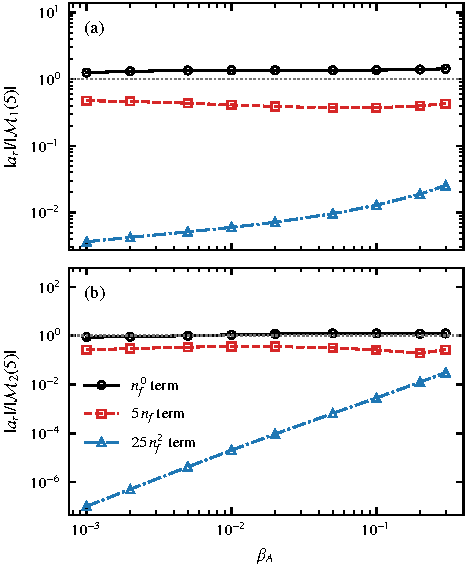
\includegraphics[width=\columnwidth]{figures/fig2_flavour.pdf}
 \caption{Magnitudes of the three terms of Eq.~\eqref{eq:nf5-sum}, divided by the magnitude of the complete coefficient, for $c=\BenchCos$, $\mA=\muR=\BenchMA\,\mathrm{GeV}$ and $\Nc=\BenchNc$. The horizontal line marks unity.}
 \label{fig:flavour-components}
\end{figure}

\begin{table}[t]
\centering
\caption{Evaluation time for the two complete Type II coefficients at the benchmark parameters, $c=\TimingCos$ and \TimingPrecision-digit working precision, for the unexpanded remainders (exact) and the series. First calls start with empty caches; repeated times are medians of \TimingRepeats{} evaluations at the same point. Starting the kernel and loading the files are excluded.}
\label{tab:timing}
\begin{ruledtabular}
\footnotesize
\setlength{\tabcolsep}{2.6pt}
\begin{tabular}{lcccccc}
& \multicolumn{3}{c}{first call [s]} & \multicolumn{3}{c}{repeated [s]} \\
$\bA$ & exact & series & ratio & exact & series & ratio \\
\hline
$1/10$ & 56.04 & 11.61 & 4.83 & 0.3422 & 0.0178 & 19.18 \\
$1/5$ & 45.68 & 11.64 & 3.92 & 0.3403 & 0.0179 & 18.99 \\
$3/10$ & 44.64 & 11.64 & 3.84 & 0.3485 & 0.0181 & 19.22 \\
\end{tabular}
\end{ruledtabular}
\end{table}



\emph{Scale dependence at two loops.} With the same ingredients, and with the subtraction operator $I^{(2)}$ of the original code, which, unlike Eq.~(3.4) of Ref.~\cite{Bhattacharya:2019bmd}, does not multiply the constant
\begin{align}
 H_g^{(2)}&=\tfrac12\Bigl[C_A^2\bigl(-\tfrac{5}{12}-\tfrac{11}{24}\zeta_2-\tfrac12\zeta_3\bigr)+C_A\nf\bigl(\tfrac{29}{27}+\tfrac{\zeta_2}{12}\bigr)
 \nonumber\\
 &\qquad-\tfrac12C_F\nf-\tfrac{5}{27}\nf^2\Bigr]
 \label{eq:H2}
\end{align}
by $(-\hat s/\muR^2)^{\epsilon}$, one finds
\begin{equation}
 \frac{\partial\Mfull{}}{\partial\ln\muR^2}=3\beta_0\,\mathcal M^{(1),\Fin}+\bigl(2\beta_1-8H_g^{(2)}-12C_F\nf\bigr)\mathcal M^{(0)},
 \label{eq:rg-two}
\end{equation}
where $\beta_1=\tfrac{34}{3}C_A^2-2C_F\nf-\tfrac{10}{3}C_A\nf$ and the last term comes from the counterterm of the $O_G$--$O_J$ amplitude, Eq.~\eqref{eq:gj-proportional}, in the renormalisation of Ref.~\cite{Bhattacharya:2019bmd}. We fitted $\partial\Mfull{}/\partial\ln\muR^2=a\,\beta_0\mathcal M^{(1),\Fin}+b\,\mathcal M^{(0)}$ to the series at two velocities and angles, for $(\Nc,\nf,\mA)=$ \RGSets. With both lines of Eq.~\eqref{eq:normalisation}, $a=\RGCoefficient$ to \RGaDev{} and $b$ agrees with Eq.~\eqref{eq:rg-two} to \RGbDev, the accuracy of the series at these velocities; the second derivative equals $6\beta_0^2\mathcal M^{(0)}$, the value implied by Eqs.~\eqref{eq:rg-one} and \eqref{eq:rg-two}, to \RGSecondDev. Without the division by \FileFactor{} the fit gives $a=\RGCoefficientPublished$, and without the scale term of the one-loop remainders $b$ differs from Eq.~\eqref{eq:rg-two} by $6\beta_0^2\ln(\mA^2/\mathrm{GeV}^2)$; the agreement therefore also fixes the reference scale of the published one-loop remainders at $\muR=1$~GeV.

\emph{Origin of the factor \FileFactor.} The Mathematica code of the original calculation documents it: the two-loop renormalisation step multiplies the $O_G$--$O_G$ amplitude, including the tree and one-loop amplitudes that enter the infrared subtraction, by $\FileFactor=\FileFactorRoot^2$, whereas the one-loop step does not. The pole cancellation of Ref.~\cite{Bhattacharya:2019bmd} is unaffected, since all terms of the two-loop subtraction carry the same factor. The released code and data use the normalisation of Eq.~\eqref{eq:normalisation}.

\emph{The original output.} The Mathematica output of the original calculation confirms both corrections. Its one-loop remainders, normalised to the tree amplitude, depend on $\muR$ as in Eq.~\eqref{eq:rg-one} and agree with the first line of Eq.~\eqref{eq:normalisation} to \ArchiveOneLoopDev; the published one-loop files coincide with them at $\muR=1$~GeV. An earlier version of the two-loop renormalisation step, without the factor \FileFactor{} and with the $O_J$ contribution switched off, was evaluated at $x=1/11$, $z=3/11$. At that point the published $P_1$ remainder equals \FileFactor{} times this result, multiplied by the tree amplitude, plus the $O_G$--$O_J$ counterterm of the published version; the real parts agree to \ArchiveTwoLoopDev. The imaginary parts differ by $32C_F$ times the one-loop $O_G$--$O_J$ amplitude, a multiple of the tree amplitude, so the two versions of the code treat this counterterm differently. In the normalisation of Eq.~\eqref{eq:normalisation} the difference is $24C_F\nf$ times the tree amplitude, which changes $\as^2V_2$ by \ArchiveOJShift; it belongs to the $O_J$ contribution discussed in Sec.~\ref{sec:rate}. The files and a script that reproduces these comparisons are part of the released material.
